\section*{Aufgabe 1}
\section{logistische Funktion}
Die Iterationsroutine kann in der Datei "Bifurkation.py" eingesehen werden. \\
Eine Möglichkeit um das $R_{max}$, also den maximalen R-Wert zu bestimmen, bei dem die Abbildung innerhalb der Grenzen bleibt, ist in der Datei "MaxR.py". Für die logistische Funktion wird ein $R_{max}$ von 4 bestimmt. \\
\begin{figure} [h]
	\centering
	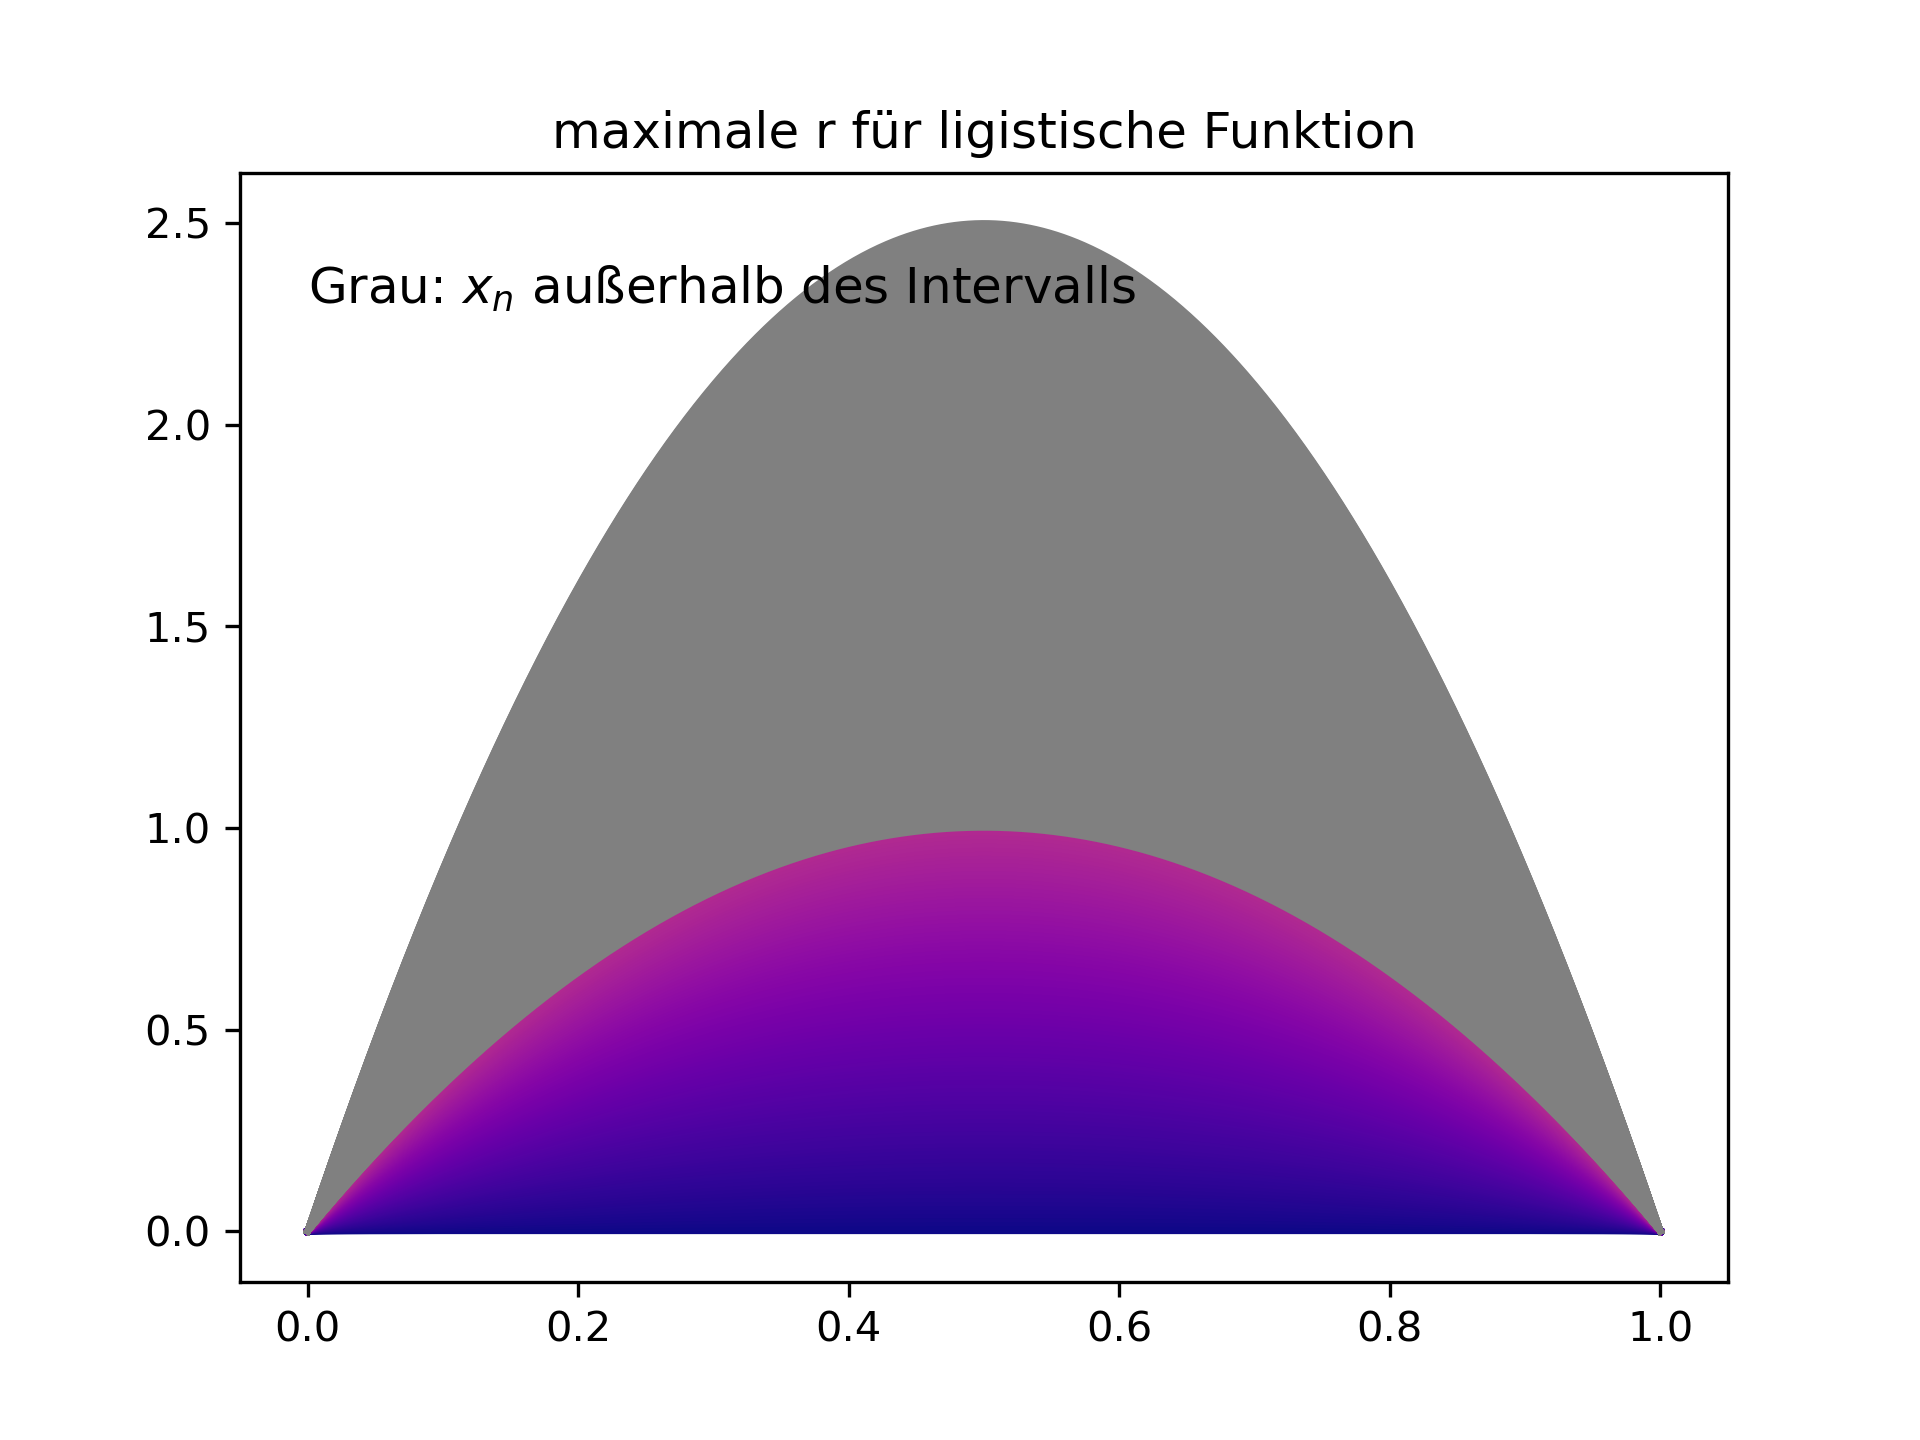
\includegraphics[width=0.5\textwidth]{Aufgabe1/logisticMaxR.png}
	\caption{Darstellung für die Bestimmung von $R_{max}$}
\end{figure}
Zur Bestimmung der Fixpunkte wird der Ljapunow-Exponent verwendet. Er ist der natürliche Logarithmus des Betrags der Ableitung und wird deswegen =0 wenn die Ableitung =1 wird. Er wird entsprechend =0 (näherungsweise) an marginal stabilen Fixpunkten (wo Fixpunkte instabil werden). Beim Plotten des Ljapunow-Exponent stellt daher die Anzahl der Nullstellen die Anzahl der Fixpunkte dar, bei denen sich die Orbits verdoppeln. Die Feigenbaumkonstante berechnet sich dann aus dem Verhältnis der Abstände dieser Nullstellen. Da $R_{\infty}$ definiert ist mit $G=64=2^{6}$, ist der chaotische Punkt ab der 5. Nullstelle des Ljapunow-Exponenten erreicht. 
Bestimmte Nulstellen:\\
\begin{center}
\captionof{table}{Nullannäherungen Ljapunow-Exponent}
\begin{tabular}{cc}
\toprule
r & Ljapunow-Exponent/Iterationen \\
\midrule
1.001 & -0.0008\\
2.999 & -0.0005\\
3.448 & -0.0011\\
3.543 & -0.0007\\
3.605 & 0.0028\\
\bottomrule
\end{tabular}
\end{center}
Daraus ergibt sich die Feigenbaumkonstante zu $\delta = 4,72$ und $R_{\infty} = 3,605$. Es wurden 4 verschiedene Startwerte verwendet. Die Abbildungen dazu sind im Ordner. Eins mit Startwert $x_0 \approx 0$ ist hier angehängt:\\
\begin{figure} [h]
	\centering
	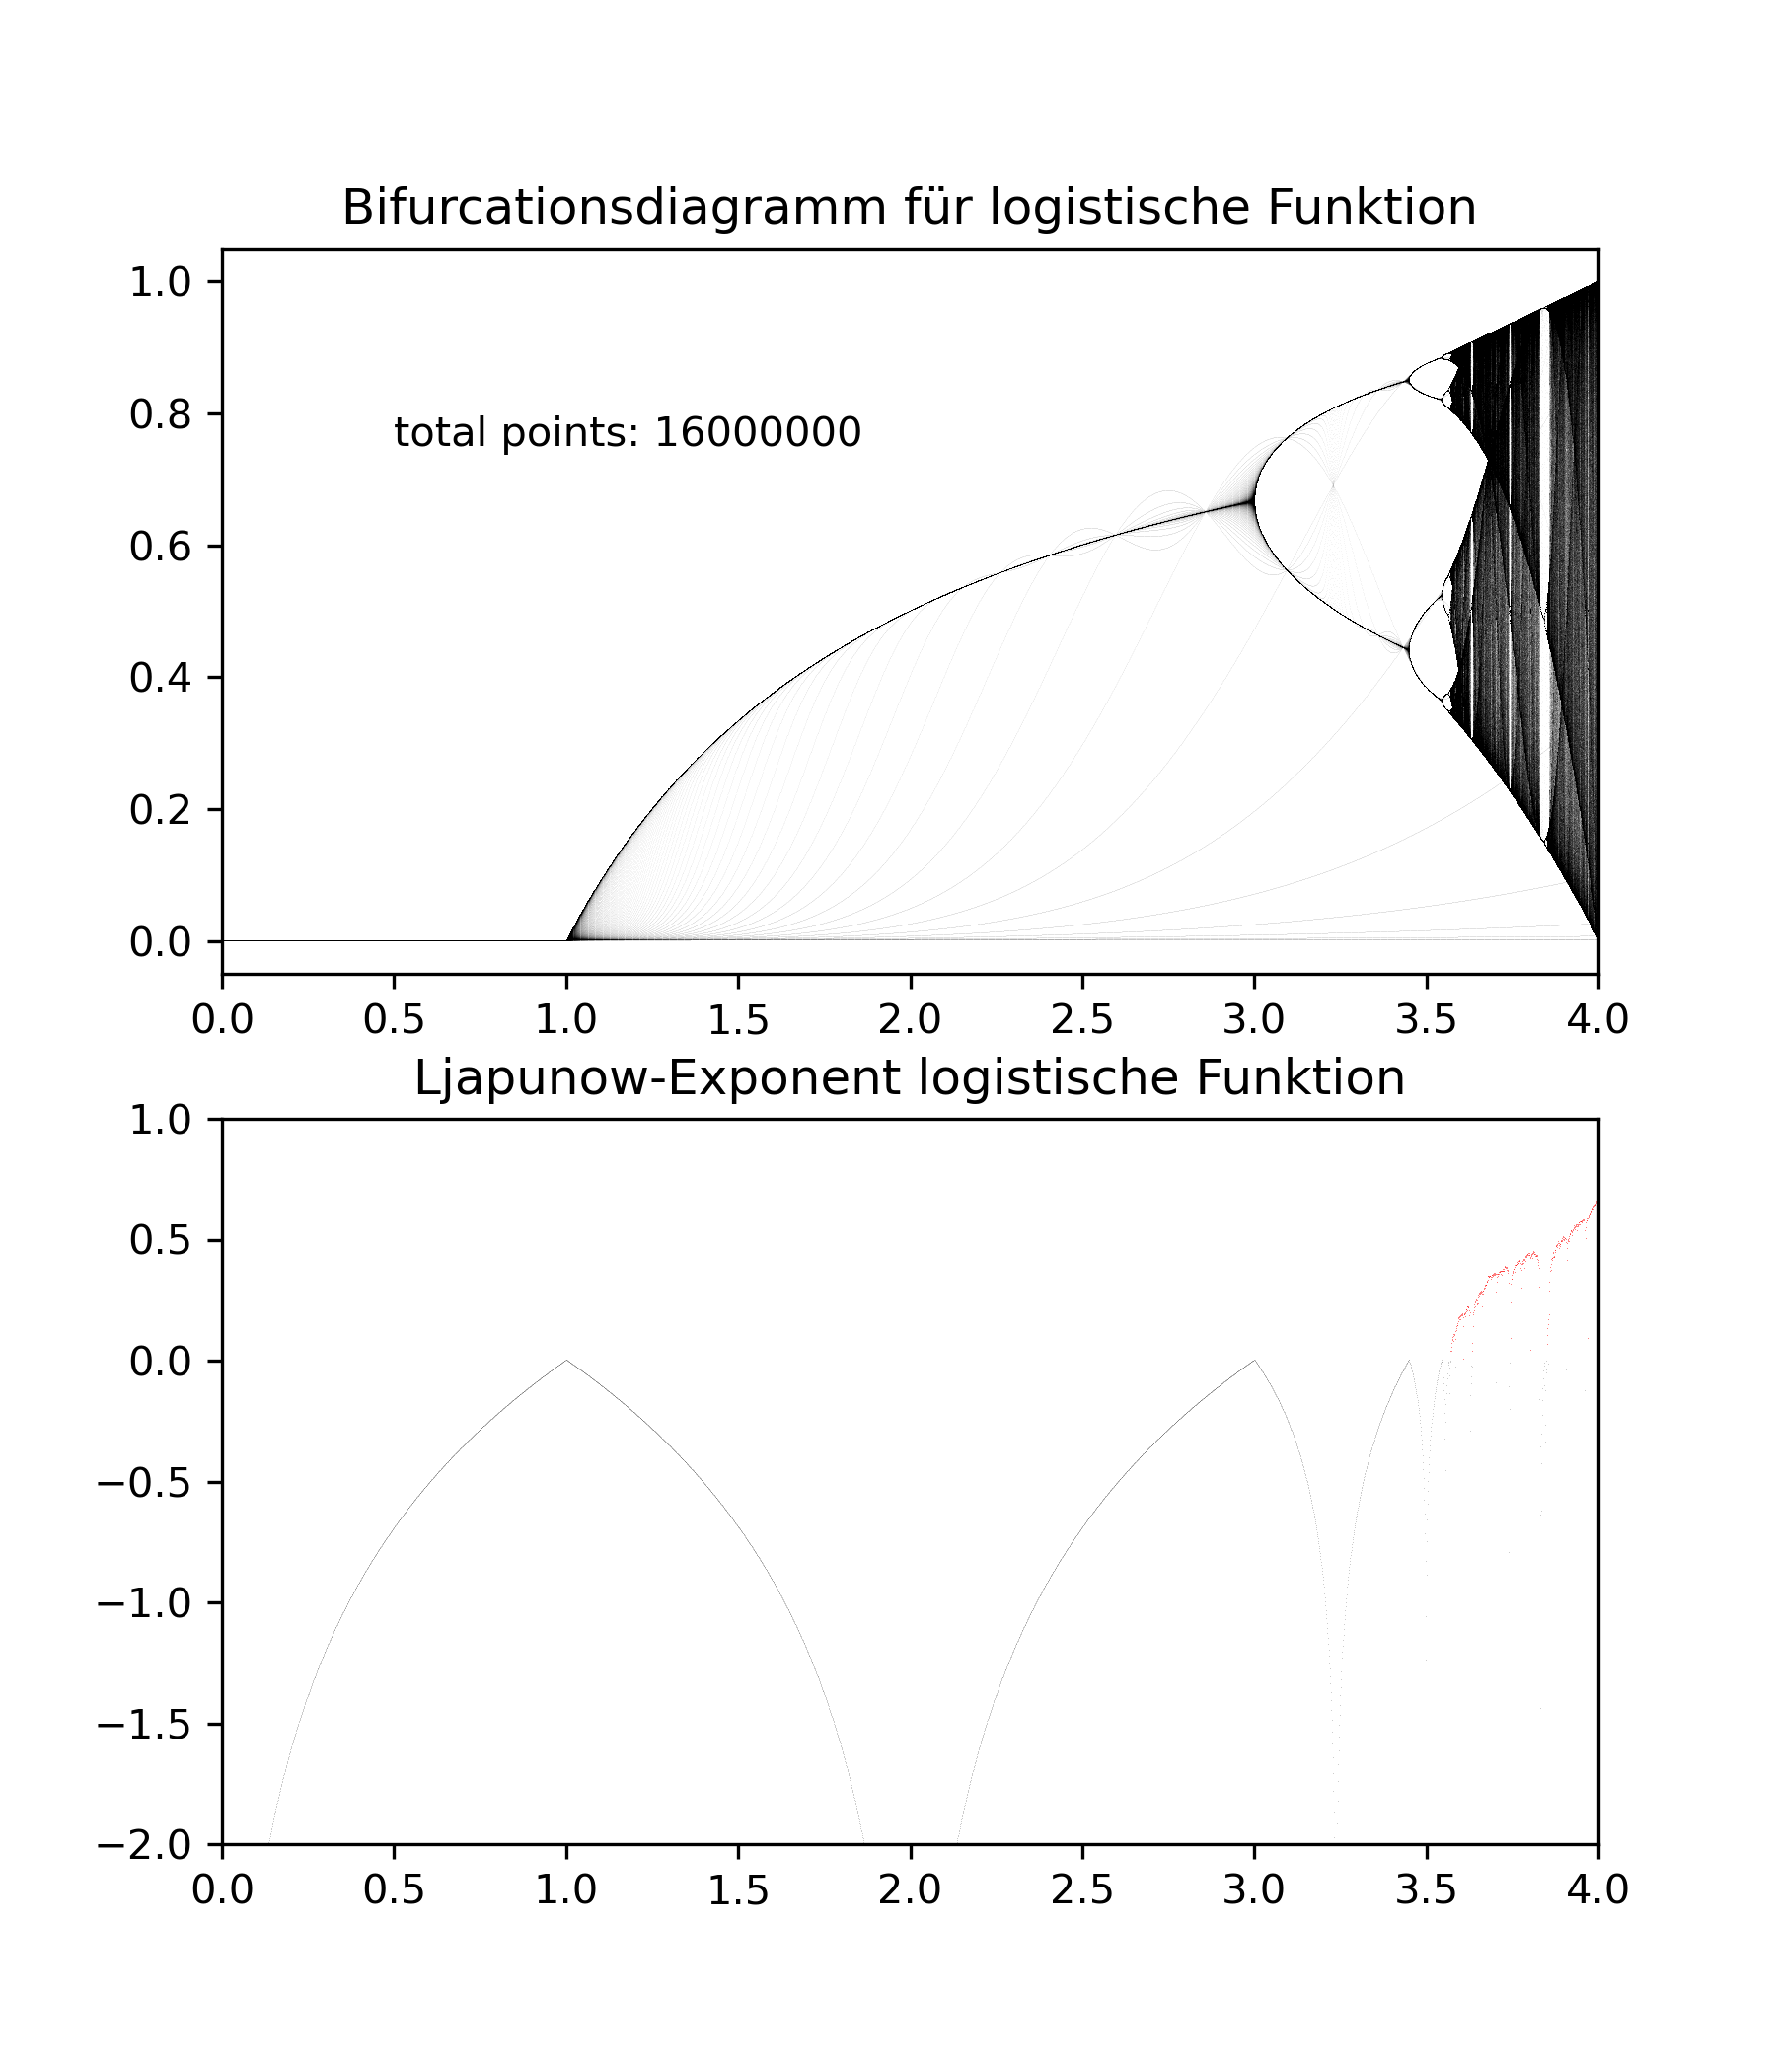
\includegraphics[width=0.5\textwidth]{Aufgabe1/logistic.png}
	\caption{Bifurkationsdiagramm logistische Funktion}
\end{figure}

\section{kubische Funktion}
Das Vorgehen bleibt natürlich das selbe wie bei der logistischen Funktion.\\
\begin{figure} [h]
	\centering
	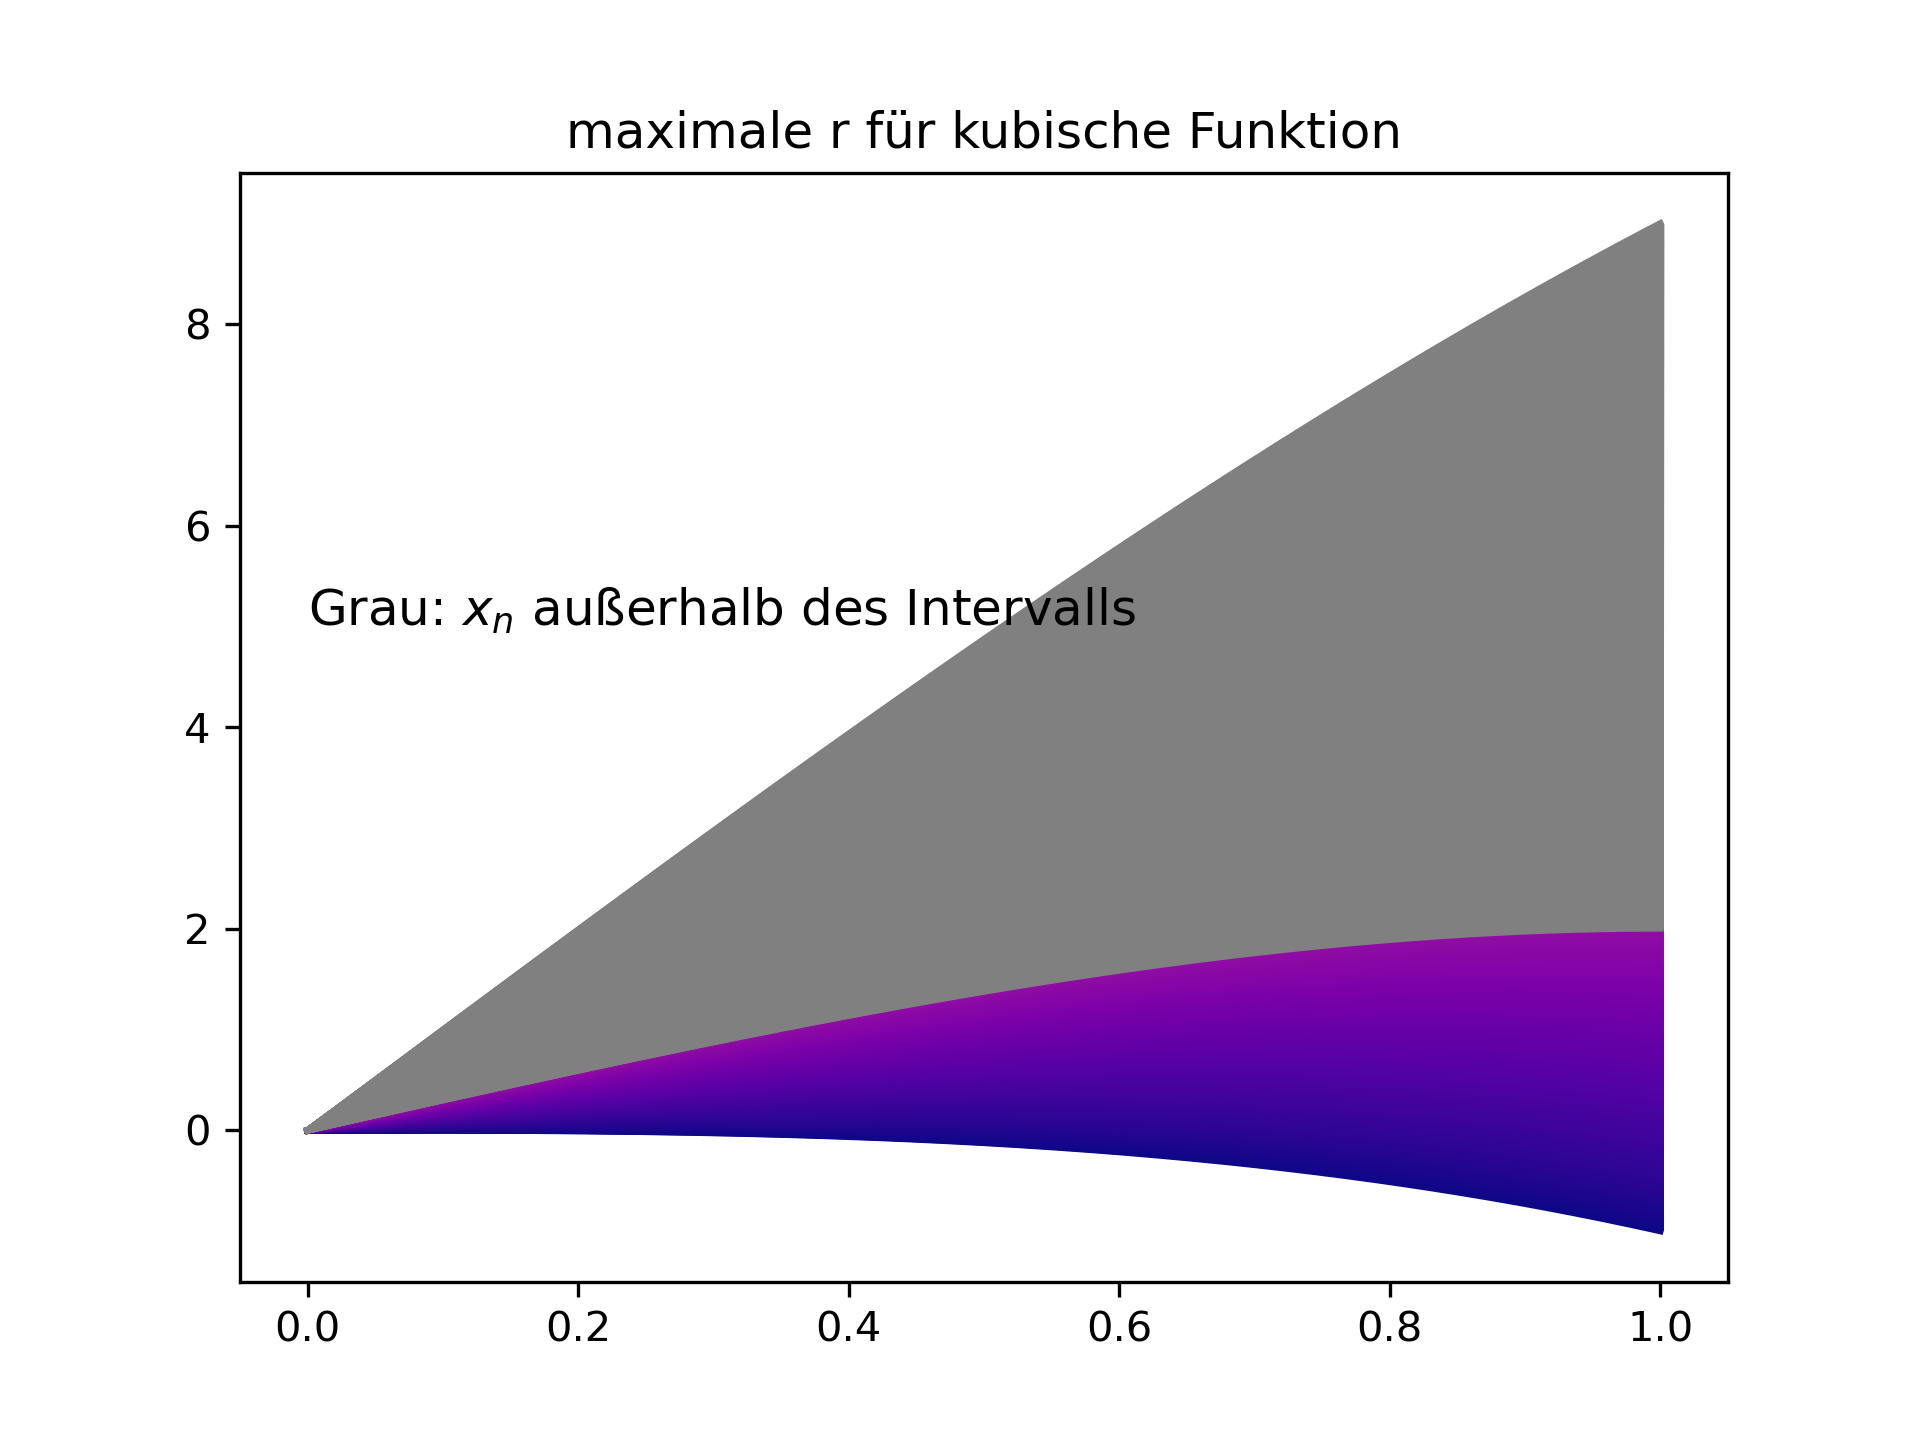
\includegraphics[width=0.5\textwidth]{Aufgabe1/kubicMaxR.png}
	\caption{Darstellung für die Bestimmung von $R_{max}$}
\end{figure}
\begin{figure} [h]
	\centering
	\includegraphics[width=0.5\textwidth]{Aufgabe1/kubic.png}
	\caption{Bifurkationsdiagramm kubische Funktion}
\end{figure}
$R_{max}$ wird bestimmt zu $R_{max} = 3$. Es ergeben sich nur 2 Nullstellen des Ljapunow-Exponenten.\\
\begin{center}
\captionof{table}{Nullannäherungen Ljapunow-Exponent}
\begin{tabular}{cc}
\toprule
r & Ljapunow-Exponent/Iterationen \\
\midrule
0.999 & -0.0006\\
1.645 & -0.0007\\
\bottomrule
\end{tabular}
\end{center}
Zur Bestimmung dvon $\delta$ und $R_{\infty}$ werden deswegen die Orbits weiteren nur abgelesen zu $r_3 = 2.25$, $r_4 = 2.3$, $r_5 = R_{\infty} = 2.31$. \\
(Bei der kubischen Funktion bin ich mir nicht besonders sicher)